\chapter{Présentation du projet}

\section{Sujet}
%Présentation du sujet : entreprise, encadrement

\par Notre objectif était de réaliser la première version d'un environnement de développement simplifié accessible depuis un navigateur web. Il devait permettre d'écrire et de compiler du code rapidement et simplement sans avoir à installer de compilateur sur le poste client (la compilation s'effectuant sur le serveur). Cet outil pourrait être utilisé, dans le cadre des enseignements à l'Université d'Angers, dans plusieurs unités dès la L1 jusqu'à la L3 (voire jusqu'au master si certaines fonctionnalités adaptées sont implémentées). \\

\par Certaines caractéristiques nous étaient demandées :

\begin{itemize}

	\item l'édition de code dans un éditeur proposant la coloration syntaxique
	\item la possibilité de compiler le code grâce à des compilateurs installés sur le serveur. Le logiciel devait prendre en compte différents langages afin d’être utilisable dans différentes UE
	\item l'accès aux messages d'erreur de la compilation
	\item l'exécution de l'application compilée sur le serveur avec affichage de la sortie
	\item des fonctionnalités avancées devaient être développées telles que l’intégration du débogueur, une gestion plus poussée de l’ensemble de fichiers composant un projet, l'auto-complétion du code, l'intégration d’outils d’analyse

\end{itemize}


\section{Problématique soulevée}

\par L'enjeu principal de ce projet était la sécurité du serveur. En effet, l'application va compiler et exécuter du code inconnu. Il faut, d'une part, empêcher qu'un utilisateur puisse obtenir des accès qu'il ne devrait pas obtenir, et aussi, gérer les inévitables programmes trop gourmands. Lorsqu'un étudiant tente d'exécuter un programme qui contient des erreurs ou qui demande trop de mémoire CPU, il ne faut pas que le serveur qui gère l'exécution ni que les exécutions d'autres étudiants soient ralenties ou bloquées. Il est donc nécessaire d'élaborer une architecture visant à répondre à ces problématiques. Nous avons décidé d'utiliser une technologie de conteneurisation pour répondre à cette problématique.

\par Le projet se devait également d'être modulable, afin de pouvoir facilement ajouter le support de nouveaux langages. À cette fin, nous avons décidé de conserver les informations liées à chaque langage supporté dans une base de données relationnelle.

\par Nous avons aussi décidé de réduire l'accès à l'application, en demandant aux utilisateurs de s'inscrire via une adresse e-mail (inscription pouvant être ouverte seulement à certaines personnes, par exemple sur la base du nom de domaine d'une adresse e-mail : cela permet d'empêcher les personnes extérieur à l'Université d'utiliser l'application, réduisant ainsi la charge sur les serveurs). Afin de pouvoir répondre plus facilement à cette problématique et à la précédente, nous avons choisi d'utiliser un framework déjà existant qui nous permettrait de faciliter la gestion de ces fonctionnalités.

\section{Choix des principaux outils et technologies}
\label{sec-principaux-outils}
\par Lors de la première séance de concrétisation disciplinaire, nos chefs de projet nous ont proposé d'utiliser le framework Symfony \footnote{Voir \url{https://symfony.com/}} pour la réalisation de notre application. Ce framework force à organiser le code et permet une gestion simple de la base de données qui ne dépend pas du type de celle-ci. En effet, Symfony intègre la bibliothèque Doctrine\footnote{Plus de détails sur \url{http://www.doctrine-project.org/}}, facilitant la manipulation de bases de données et permettant le mapping d'une base de données relationnelle avec des objets PHP. De plus, Symfony permet une génération simple des pages grâce à ses contrôleurs et au moteur de templates twig. L'autre avantage qui nous a décidé à choisir Symfony est la possibilité d'utiliser des bundles (par exemple, FOSUserBundle permet la gestion des utilisateurs) qui simplifient et accélèrent véritablement la réalisation des projets. \\

\par Nous avons choisi d'utiliser MariaDB comme système de base de données. MariaDB est l'un des systèmes de gestion de base de données les plus importants et a l'avantage d'être distribué sous licence libre. De plus, cet outil est soutenu par une large communauté, ce qui assure une maintenance sur le long terme. Néanmoins, ce SGBD\footnote{Système de Gestion de Base de Données} peut facilement être remplacé par un autre au besoin, puisque toutes les manipulations de base de données se font via l'ORM\footnote{Object-Relationnal Mapping} de Symfony. Le seul pré-requis est que le SGBD soit supporté par Doctrine. \\

\par Bootstrap\footnote{Voir \url{https://getbootstrap.com/}} est un framework HTML/CSS/JS simple d'utilisation. Il utilise un layout sous la forme d'une grille qui s'adapte en fonction de la taille de l'écran. Il inclut aussi un style de base pour tous les éléments HTML, ce qui permet d'obtenir un style indépendant du navigateur ou de l'OS utilisé par l'utilisateur. Ce style peut également être modifié via des constantes SASS\footnote{Syntactically Awesome Stylesheets} si on souhaite aller plus loin dans la personnalisation de l'application.
\par Enfin, Bootstrap possède de nombreux composants faciles à manipuler via des attributs HTML (ou via le Javascript) tels que les dropdowns, modals, alert... \\

\par La conteneurisation, et plus particulièrement Docker\footnote{\url{https://www.docker.com/}}, s'est vite imposée dans l'architecture du serveur. Docker est une méthode de conteneurisation légère qui permet de travailler toujours sur le même environnement (la même image est réutilisée autant de fois que nécessaire) et qui nous a permis d'isoler les compilations et exécutions des programmes.

\section{Répartition des tâches}

\par Afin de travailler efficacement, nous avons séparé le projet en 4 parties plus ou moins autonomes: Paulin s'est occupé de l'interface graphique, Yassine de l'administration, Jérôme de l'architecture du serveur et Valentine de la communication entre les serveurs.

\begin{figure}[H]
\centering
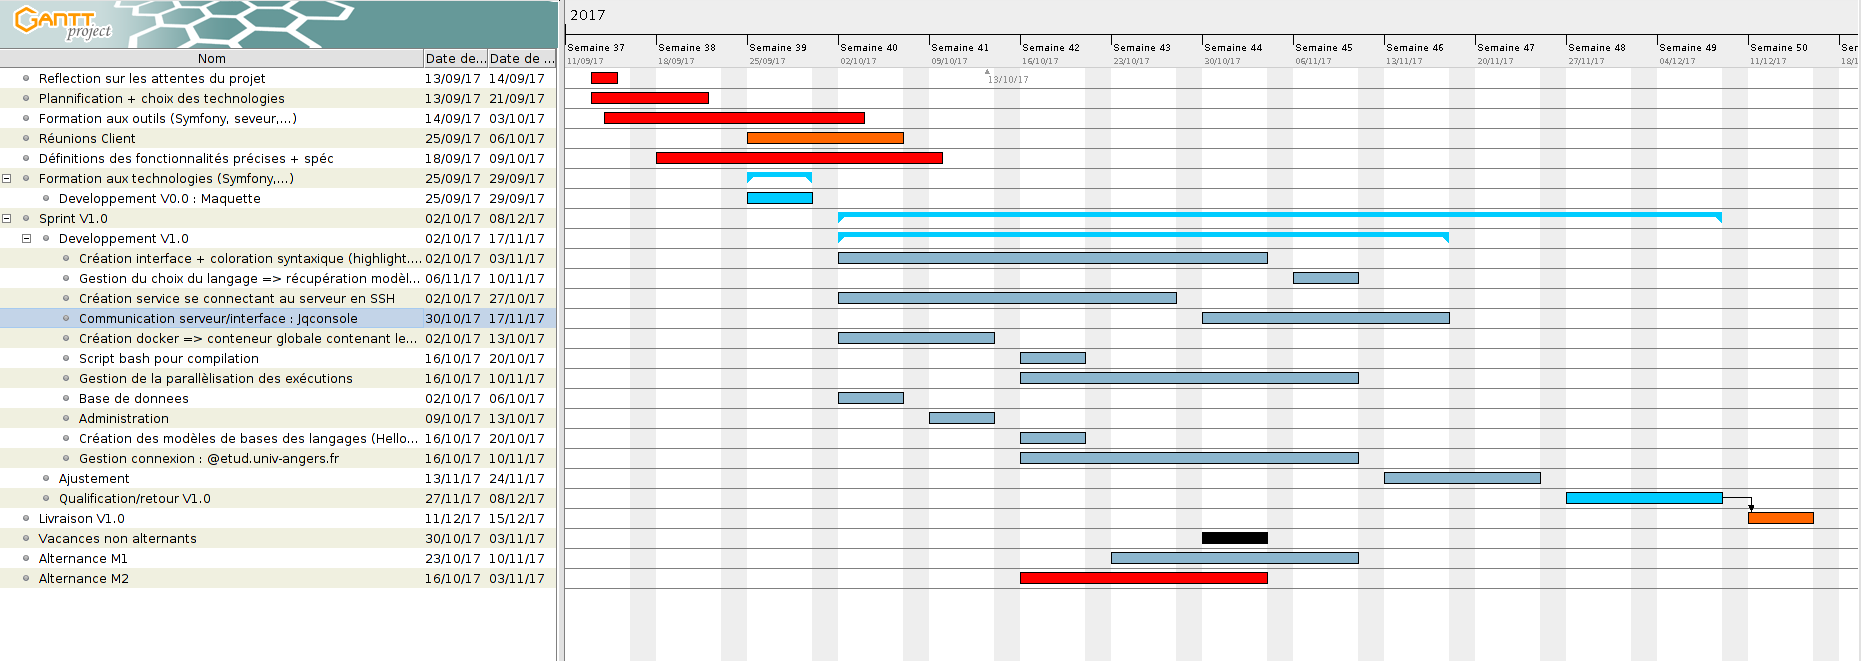
\includegraphics[width=1\textwidth]{./img/gantt_LIDE.png}
\caption{Planning}
\end{figure}
